\documentclass[
	a4paper,%
	11pt,% <10pt, 9pt>
	]{article}
	
\usepackage[english]{babel}
\usepackage{graphicx}
\usepackage{subcaption}
\usepackage{tabularx}
\usepackage{booktabs}
\usepackage{hyperref}

	
	
\begin{document}

\title{Roles feature in Karrot - Writeup of process}

\author{Nathalie Szycher}
\date{\today}

\maketitle
\tableofcontents


\section{Introduction}

This writeup covers the process to design and implement a roles feature and fine-grain of the activities configuration in Karrot. Karrot is a free and open-source software project run by community. It originated from a food saving movement, therefore many active groups are in this field of action. Although there are more groups joining with different aims then food saving, they all still relate to some concepts of Commoning.

Karrot is a software to help groups in particular grassroot initiatives to organise and build a community. One of the core features is the possibility to set up activities where volunteers within a Karrot group can sign up for. Over time groups develop more advanced processes for onboarding or specific needs in order to successfully do an activity. To support the groups organising an ongoing development and iteration of the software is needed.

One part of the new feature is to allow more customisation when setting up an activity. Who is taking the cargo bike? How many people do we need for cutting vegetables and who is doing the cooking? The other part is to allow limitation of certain activities to specific user groups so called roles. The following sections will cover more background information, the drivers to work on these features and how they've been designed and implemented. This is part of the milestones for Karrots funding from NGI0 Discovery Fund established by NLnet.



\section{Background}

Karrot is well suited for food saving and sharing activities, so this example will guide us through the software. Nevertheless the features can be easily adapted for other types of activities and actions groups can possibly do. One core function to help coordination within a group is the activity feature. It is used for example to coordinate food pickups from stores. Places are used to display stores and within a place different activities can be set up. Group members can now self-assign for doing the activity. An example is shown in \autoref{fig:screenshot-pickup}.

\begin{figure}[ht]
	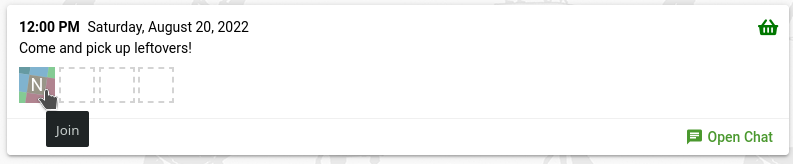
\includegraphics[width=\textwidth,
	]{images/screenshot_pick-ups.png}
	\caption{Screenshot of sign-up for pickups in Karrot}
	\label{fig:screenshot-pickup}
\end{figure}

Within a Karrot group there are several roles which come with the software (see \autoref{tab:roles_karrot_current}). Whereas everyone is a group member, the newcomer and editor roles depend on trust given to the user. Newcomer is the default role for someone joining the group. It allows the person to join any activity in the group. As the name suggests, editors have additional rights to add, change and remove activities. 


\begin{table}[ht]
	\centering
\caption{Current Karrot roles in a group and their explanation}
	\begin{tabular}{p{.2\textwidth} p{.4\textwidth} p{.3\textwidth}}
		\toprule
		Role & How to get there & What they can do (regarding activities)\\
		\midrule
		Group member & Being the first one in a group or if application gets accepted & - \\
		Newcomer & Below trust threshold  & Join any activity \\
		Editor & Trust threshold reached & Join any activity, edit any activity\\
		\bottomrule
	\end{tabular}
\label{tab:roles_karrot_current}
\end{table}	

Within a Karrot group persons can give trust to each other. This is indicated by a carrot icon as shown in the profile in \autoref{fig:screenshot-give-trust}. Trust can be given and revoked. Per person there is one trust to give and it is counted how many trust group members receive from others. Once a certain threshold is reached, the user gets the editor role, giving them editing permissions for the group. Depending on the group size there are different thresholds to gain editor role. The numbers are shown in \autoref{tab:roles_karrot_numbers}. Group members with less trust than the threshold stay in newcomer role. For more than 6 active group members the default value is three trust to gain editor role and have editing permissions in the group.



\begin{figure}[ht]
	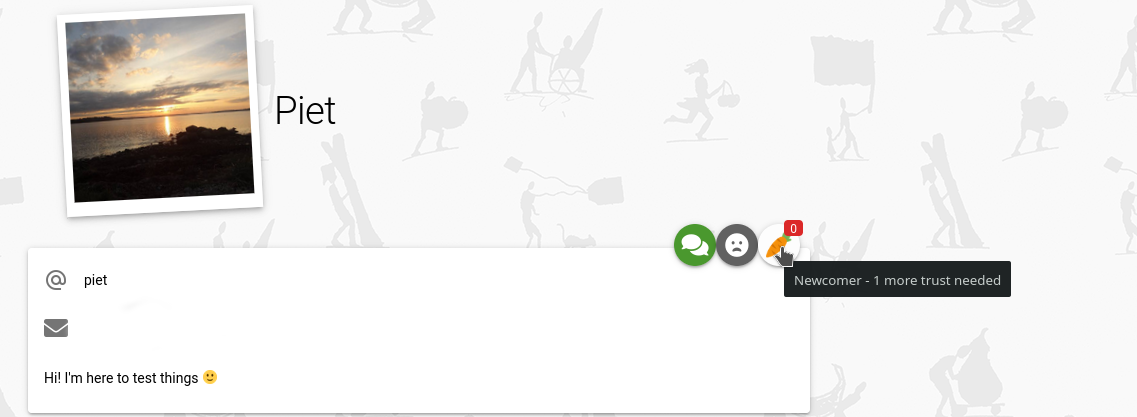
\includegraphics[width=\textwidth,
	]{images/screenshot_giving-trust-profile.png}
	\caption{Screenshot of profile and possibility to give trust to user}
	\label{fig:screenshot-give-trust}
\end{figure}



\begin{table}[ht]
	\centering
\caption{Number of trust needed for editor role depending on group size}
	\begin{tabular}{ll}
		\toprule
		Active group members & Number of trust\\
		\midrule
		1 or 2  & one trust \\
		3 or 4  & 2 trust \\
		6 or more & 3 trust\\
		\bottomrule
	\end{tabular}
\label{tab:roles_karrot_numbers}
\end{table}	


\section{Feature Design}

Feature design in Karrot usually follows a community design process inspired by the Google Sprint\footnote{\label{url_google_sprint}\url{https://www.thesprintbook.com/}}. It covers five stages from mapping to testing and is well suited for conceptualising features. Another way to design and implement a new feature is to follow a needs-based iterative approach. In that case there often is a specific driver from the community to solve a problem they are facing. In order to build software that helps the groups in their organising, it is necessary to understand their need, generate a proposal, decide on a way to go forward and implement it. Still, the stages are not that clearly defined and going back and forth between different stages is possible.

% REF TO SOCIOCRACY??

\subsection{Understand the need}

The initial prompt is coming from a Karrot group in Luxembourg which is using Karrot to organise their food saving and sharing activities. The conversation started back in November 2020 in the Karrot community forum\footnote{\label{url_forum_2020}\url{https://community.karrot.world/t/applicant-trial-pickup-proposal/575}}. This group is having a specific  onboarding process. In order to join group activities in the future, a person coming into the group first needs to do three so-called trial pick-ups. These are pick-ups where the new person accompanies a more experienced group member. When the trial pick-ups are successfully done, the new person is fully onboarded and can join any activity the group offers. Many other groups are having similar onboarding rules. 

Additionally pick-ups often need more advanced organising than 'come and pick up the food'. When the quantities are big, the group wants to make sure that the volunteers have enough capacities to carry the food. Some groups define requirements for certain places like 'there needs to be at least one person with big transport capacities (e.g. cargo bike/ car)'. 

What the Karrot software isn't supporting yet:
\begin{itemize}
    \item mark specific activities as suitable for trial pick-ups
    \item limit access to activities to certain user groups
    \item advanced organising of pick-ups
\end{itemize}

When looking at needs, we don't want to forget that the Karrot project itself and the development team come up with a certain set of needs themselves. They want to make a coherent story how the software works and have an eye on future and past ideas. Additionally the implementation needs to work well from a code perspective.

Taking all perspectives into account, the following are examples of a need statement:
\begin{itemize}
    \item We want to support an onboarding process within the software.
    \item We want a more advanced way to configure activities.
    \item We want to build on existing ideas and integrate it nicely into existing code.
\end{itemize}

\subsection{Generating a proposal}
	
The proposal generation went through different stages and turns, which won't be discussed in detail. Early on it was clear that the requested changes touch the topic of roles in Karrot and with that how the trust system in Karrot works. Splitting the topic into two parts helped to stay on track and bring the work towards closure. The first part is to build a feature soon that is helpful for the groups and fulfils the needs identified. This is the scope of this work. The second part is to do a full community design process on group governance and roles which is further discussed in \autoref{sec:outlook}. The following is a description of the synthesized feature proposal.


\begin{itemize}
	\item There is the possibility to customize activities
	\begin{itemize}
		\item Entering an advanced mode
		\item Possibility to define different participant types with custom descriptions
	\end{itemize}
	\item Trust system features another role called 'approved'
	\item Sign-up for activities can be limited based on the role of the user
	\begin{itemize}
		\item When not using the advanced mode for activities, anyone can sign up to activities
		\item When using the advanced mode for activities it is possible to define per activity which user group is eligible if signing up
	\end{itemize}
\end{itemize}


A summary of the new proposed Karrot roles is shown in \autoref{tab:roles_karrot_new}. The main difference is the addition of the role called 'approved'. Group members who have this role can sign in for activities that are set for approved-only or anyone. The numbers of trust needed for 'approved' are shown in \autoref{tab:roles_karrot_numbers_new} which is one trust independent of the group size. Note that only editors can give other users trust for 'approved'!


\begin{table}[ht]
	\centering
\caption{New Karrot roles in a group and their explanation}
	\begin{tabular}{p{.2\textwidth} p{.4\textwidth} p{.3\textwidth}}
		\toprule
		Role & How to get there & What they can do (regarding activities)\\
		\midrule
		Group member & Being the first one in a group or if application gets accepted & - \\
		Newcomer & Below trust threshold for \newline editor and approved & Join activities open for anyone or newcomer \\
		Approved & Trust threshold reached for \newline approved & Join activities open for anyone or approved \\
		Editor & Trust threshold reached for \newline editor & Join activities open for anyone or editor, edit any activity\\
		\bottomrule
	\end{tabular}
\label{tab:roles_karrot_new}
\end{table}	

\begin{table}[ht]
	\centering
\caption{Number of trust needed for editor and approved role depending on group size}
	\begin{tabular}{p{.3\textwidth} p{.3\textwidth} p{.3\textwidth}}
		\toprule
		Active group \newline members & Number of trust for \newline editor & Number of trust for \newline approved\\
		\midrule
		1 or 2  & one trust & one trust \\
		3 or 4  & 2 trust & one trust \\
		6 or more & 3 trust & one trust\\
		\bottomrule
	\end{tabular}
\label{tab:roles_karrot_numbers_new}
\end{table}	
	
\subsection{Decide}

As mentioned above the process for designing this feature went through many stages and had periods of more or less activity in the last two years. As part of the NLnet milestone agreement the work was resumed. Decisions were made in incremental steps involving the people who are actively working on this topic and the users of Karrot who wanted that feature. Main communication happened over the community forum where at several occasions the state of the work was presented, receiving positive feedback\footnote{\label{url_forum_feedback}\url{https://community.karrot.world/t/applicant-trial-pickup-proposal/575/59}}. The second instance to receive feedback is the 'Karrot team'. Following the iterative approach, the above proposal is the current state of the decision process. The feature will be marked with a tag, so it can be activated per group on demand.

 
\subsection{Implement}

From a technical perspective the development needs changes both on Frontend and Backend level. Also the work is divided into two parts, reworking how activities are configured and adding trust for another (in this case 'approved') role. Here are the references to the respective github pull requests:
\begin{enumerate}
    \item Activities configuration
    \begin{itemize}
    		\item Fronted: Activities that require role\footnote{\label{url_github_2421}\url{https://github.com/karrot-dev/karrot-frontend/pull/2421}}
    		\item Backend: Add activity roles\footnote{\label{url_github_1199}\url{https://github.com/karrot-dev/karrot-backend/pull/1199}}    
    \end{itemize}
    %\newpage
    \item Trust for role
    \begin{itemize}
    		\item Frontend: Trust for role\footnote{\label{url_github_2589}\url{https://github.com/karrot-dev/karrot-frontend/pull/2589}}
    		\item Backend: Add trust for role\footnote{\label{url_github_1167}\url{https://github.com/karrot-dev/karrot-backend/pull/1167}}
    \end{itemize}
\end{enumerate}

From a user perspective the interface how to join activities changed. When different participant types are enabled the user sees the custom description and which role is needed in order to join (see \autoref{fig:screenshot-pickup-roles}). From an editing perspective it is configurable whether participant types are used or not. When using the participant type toggle editors can add information, set the number of slots and define to which role it's open as shown in \autoref{fig:screenshot-create-role}.

\begin{figure}[!h]
\centering
\begin{subfigure}{0.55\textwidth}
\centering
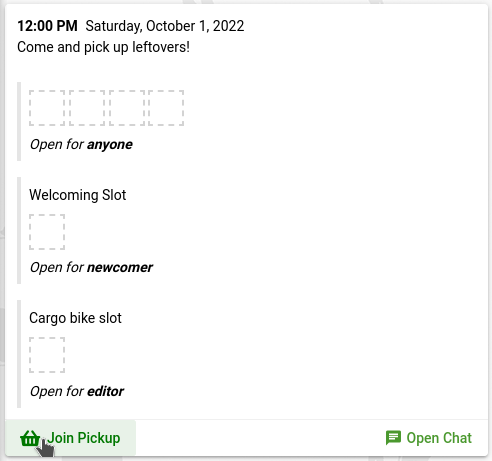
\includegraphics[width = \textwidth]{images/screenshot_pick-ups_roles.png}
\caption{Overview of activity}
\end{subfigure}
\begin{subfigure}{0.44\textwidth}
\centering
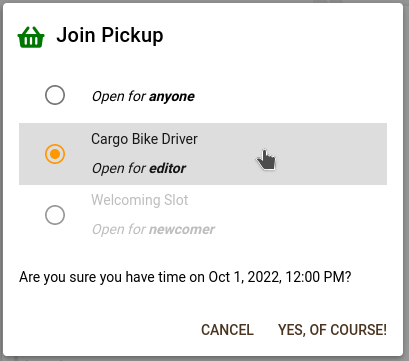
\includegraphics[width = \textwidth]{images/screenshot_pick-ups_roles_join.png}
\caption{How to join}
\end{subfigure}
\caption{Screenshot of sign-up for pickups in Karrot with custom participant types}
\label{fig:screenshot-pickup-roles}
\end{figure}

\begin{figure}[!h]
	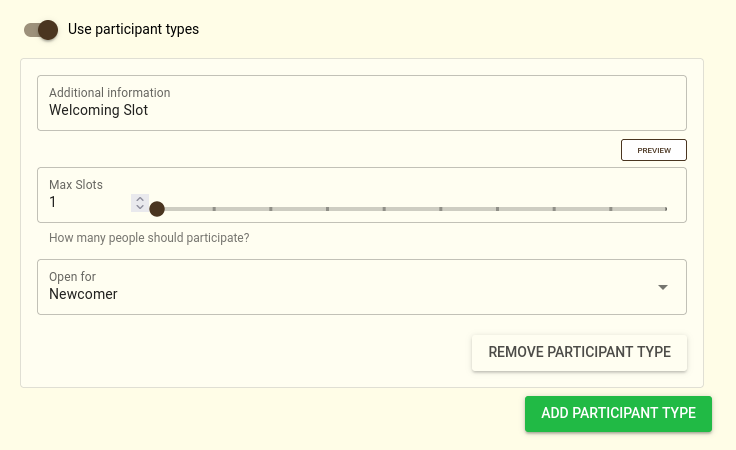
\includegraphics[width=0.97\textwidth,
	]{images/screenshot_pick-ups_participant-type.png}
	\caption{Screenshot of how to create a new participant type for an activity}
	\label{fig:screenshot-create-role}
\end{figure}


To explore how the 'trust for approved' feature can be integrated on a member's profile page, different designs were made with the open-source design and prototyping platform https://penpot.app/\footnote{\label{url:penpot_designs}\url{https://community.karrot.world/t/applicant-trial-pickup-proposal/575/63}}. The implemented design is shown in \autoref{fig:screenshot-give-trust-roles}. On a group member's profile page another button is added. The button with the carrot icon is still prompting the same behaviour to give trust for editor role. Now the second button with the leaf icon is there to give trust for approved role. This minimal design was chosen to have high compatibility across groups, as this feature can be enabled on request of the group. The participant types change for every Karrot group as this feature can also be used without having an 'approved' role.

\begin{figure}[!ht]
	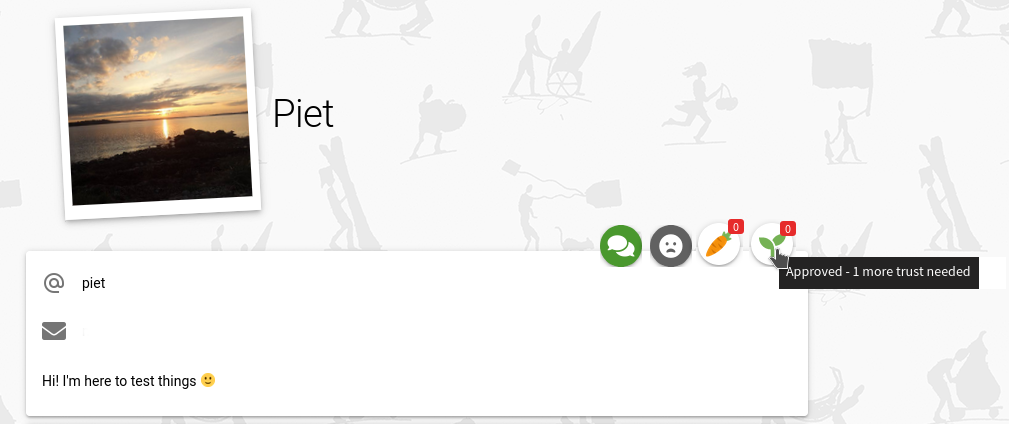
\includegraphics[width=\textwidth,
	]{images/screenshot_giving-trust-profile_approved.png}
	\caption{Screenshot of profile and possibility to give trust to user for both editor and approved}
	\label{fig:screenshot-give-trust-roles}
\end{figure}


Special care needs to be taken when editing existing activity series. With new participant types in place and the option to limit certain activities to roles, it might happen that at some point a user is no longer fulfilling the criteria needed. So when a Karrot group defines an activity series with e.g. three participant types and then an editor removes one participant type, here is what happens: the editor gets a warning if group members are signed up to slots that will be removed due to the changes. It is required to fill out a custom message and explain the change. This message will be sent to the affected users telling them that the activity they signed up for is no longer available. Additionally the message is saved in the group's history (see \autoref{fig:screenshot-history}).

\begin{figure}[ht]
\centering
\begin{subfigure}{0.44\textwidth}
\centering
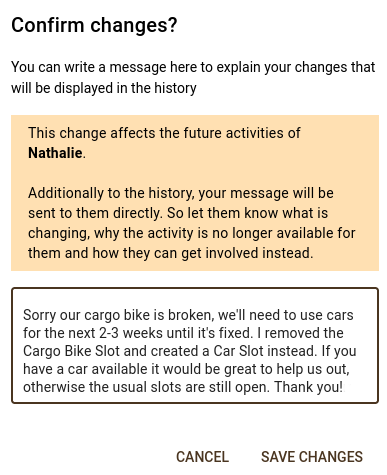
\includegraphics[width = \textwidth]{images/screenshot_activities_confirm-changes.png}
\caption{Prompt to explain changes}
\end{subfigure}
\begin{subfigure}{0.55\textwidth}
\centering
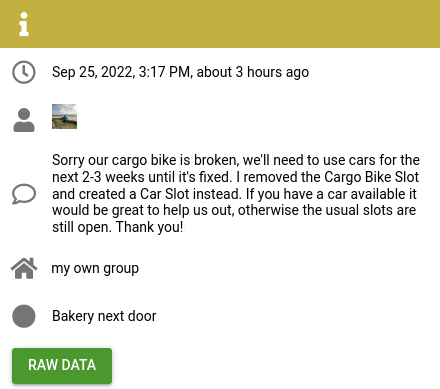
\includegraphics[width = \textwidth]{images/screenshot_activities_history.png}
\caption{History with personal message}
\end{subfigure}
\caption{Screenshot of new message box when changing activity series}
\label{fig:screenshot-history}
\end{figure}


\newpage


\subsection{Challenges}


Without doing a more formalised community design process, it is a challenge to find the right balance between conceptualising an overarching vision and concrete work to fulfil a group's need. The use of the trust system and the terminology of 'roles' can be further discussed and aligned. It is an open question how much Karrot promotes certain types of group governance and if so, which ones. Roles are a concept widely used in frameworks like sociocracy. The implementation of Karrot roles at this state doesn't follow a specific theory, it rather features an advanced way of handling permission.

The iterative and rather fluid approach and the long design period made it at times hard to follow the discussion or difficult for new team members to join. Decisions haven't always been made explicit and written down into minutes. Therefore it is challenging to see which parts of the feature are still open to discussion. Although it might be rewarding to question earlier decisions or directions, it also leads to demotivation and frustration when too many questions are opened along the way.

In addition, being very agile implies challenges to the way code is written to make sure that future iterations can build upon existing code. In this case the challenge is to implement a new feature that is compatible with all Karrot groups and their different needs. Overall the new feature should make a consistent story with existing features (editor role, activities, trust system) and the general spirit and value of the Karrot project.


\section{Conclusion and Outlook} \label{sec:outlook}

In an iterative and needs-based design process started in November 2020 from users of Karrot a set of new features were developed and implemented. Activities, which are a core functionality to many Karrot groups, have a new advanced mode where custom participant types can be configured. On group level a new role was introduced called 'approved', next to the existing 'group member', 'newcomer' and 'editor'. In the participant types menu, signing up for activity slots can be limited to certain roles.

One example where this is useful are so-called trial pick-ups often used in food saving and sharing groups. These groups don't want every new person to be able to sign up to any available slot, but have a defined onboarding process where a new group member accompanies more experienced group members first. The approved role was integrated into the trust system. Whereas any group member can give other group members trust for editor role, only editors can give other group members trust for approved. Overall this feature was designed in close interaction with the Karrot community, trying to understand their needs and making it fit into the general design of Karrot.

There is great potential to explore the use of roles in Karrot further and at some point have roles that the Karrot groups can implement themselves. This would be a good topic for a community design process, which was used before in the Karrot project. Also questions around the voting mechanism for roles and the trust feature itself can be explored further. 
More specifically the parts of this feature which are marked with a feature flag and are optional for groups, are going to be further developed and introduced to the whole community at some point. Parts of this write-up will be used to build a coherent manual of the Karrot software.



\end{document}
	
	
	